\documentclass[11pt,a4paper]{article}
\usepackage[margin=24mm]{geometry}
\usepackage[T1]{fontenc}
\usepackage{lmodern,microtype,amsmath,amssymb,amsthm,mathtools}
\usepackage{graphicx,booktabs,array,enumitem,xcolor,hyperref,fancyhdr}
\definecolor{navy}{HTML}{195C85}
\hypersetup{colorlinks=true,linkcolor=navy,urlcolor=navy,citecolor=navy,
pdftitle={The cost of inferring equilibrium before relaxation},
pdfsubject={A joint horizon, rate-range and accuracy law with an attainable experiment}}
\setlength{\parindent}{0pt}
\setlength{\parskip}{5pt}
\setlist{itemsep=3pt,topsep=5pt}
\pagestyle{fancy}\fancyhf{}
\fancyhead[L]{\small Equilibrium inference before relaxation}
\fancyhead[R]{\small 5 November 2026}
\fancyfoot[C]{\thepage}
\setlength{\headheight}{14pt}
\newtheorem{theorem}{Theorem}
\newtheorem{lemma}{Lemma}
\newtheorem{corollary}{Corollary}
\newcommand{\E}{\mathbb E}
\newcommand{\Prob}{\mathbb P}
\newcommand{\KL}{D_{\mathrm{KL}}}
\newcommand{\id}{\mathrm{id}}
\newcommand{\TV}{\mathrm{TV}}
\newcommand{\norm}[1]{\left\lVert#1\right\rVert}
\title{\textbf{The cost of inferring equilibrium\newline before relaxation}\\[5pt]
\large A joint horizon, rate-range and accuracy law\\
with an attainable experiment and exact rational compiler}
\author{Astra research construction and reproducibility record}
\date{5 November 2026}
\begin{document}
\maketitle
\begin{abstract}
We determine, up to universal constants in its logarithm, the minimum squared-drive effort needed to infer a normalized static response from short experiments on an unknown reciprocal passive relaxation system. The controller may use arbitrary causal forcing, feedback, unlimited computation and independent reset trials. For spectral ratio $\kappa$, maximum transient age $s=\mu T$, and absolute accuracy $\varepsilon$, the controlling scale is
\[
\Phi(s,\kappa,\varepsilon)=\sqrt\kappa\log(1/\varepsilon)
\log\!\left(1+\frac{\log(1/\varepsilon)}{s\sqrt\kappa}\right).
\]
Positive finite moment-matched spectra give the lower bound. A bounded monotone ramp, finite integrated readouts and a Chebyshev residual give the matching upper bound. A rational enclosure makes the implemented bias and noise certificates exact. Preparation, finite slew, calibration, repeated specimens and reuse are accounted for separately. This is a theoretical resource law within a specified interface, not a practical acceleration beyond optimal ordinary extrapolation. Historical novelty and civilisation-changing impact are not established.
\end{abstract}

\section{Question, result and scientific status}

The chosen question is operational: \emph{Can an experiment determine a system's eventual response without waiting for its slow modes, and what must replace that waiting?} The target is one static functional, rather than a reconstruction of hidden states or an entire dynamical law.

The completed result gives a matching answer in a broad but structured class. It includes an estimator that actually uses bounded forcing and finite readout windows, and a converse applying to every permitted adaptive controller. A finite upper relaxation rate changes the answer: at fixed accuracy and fixed rate range, the price of shortening the observation horizon is polynomial in $1/T$. The exponential $\exp[\Theta(1/T)]$ regime requires a family whose allowed fastest rate and hidden order can grow.

The underlying approximation and optimal-recovery ideas are established mathematics. Brown and Grabovsky's completely monotone extrapolation theorem is especially close prior work \cite{brown}; reciprocal minimax approximation is classical \cite{kraus}; and optimal recovery already connects linear functional estimation to indistinguishable pairs \cite{donoho}. The proposed contribution here is the uniform joint resource law and its fully specified acquisition operation. The literature search does not establish priority.

The proof was developed through independent construction and challenge, then checked internally by a third mathematical route. Executed numerical checks corroborate finite instances. They are not formal verification, external peer review or physical measurements. The research mission of civilisation-changing discovery has not been achieved by this scoped theorem.

\section{Model, access and resource being optimized}

Consider an unknown finite-dimensional system
\begin{equation}\label{eq:model}
\dot x=-Ax+bu,\qquad y=b^\top x,\qquad
A=A^\top,\quad \mu I\preceq A\preceq\Lambda I,\quad \norm{b}_2=1.
\end{equation}
The dimension, eigenvalues and observable weights are unknown. The normalization and bounds $0<\mu\leq\Lambda$ are supplied, certified information. The energy identity
\begin{equation}
\frac{d}{dt}\frac{\norm{x}_2^2}{2}=-x^\top Ax+uy
\end{equation}
establishes passivity. By the spectral theorem the impulse response is
\begin{equation}
k_\nu(t)=\int_\mu^\Lambda e^{-\lambda t}\,d\nu(\lambda),
\qquad \nu([\mu,\Lambda])=1,
\end{equation}
and the desired dimensionless static gain is
\begin{equation}\label{eq:target}
S(\nu)=\mu b^\top A^{-1}b
=\int_\mu^\Lambda\frac{\mu}{\lambda}\,d\nu(\lambda)\in[1/\kappa,1],
\qquad\kappa=\Lambda/\mu.
\end{equation}
An unbounded-rate class means the union of finite-dimensional realizations with no supplied common $\Lambda$; it does not require a physically infinite device.

Each mathematical trial starts at $x=0$ and has duration at most $T$. Its readout is
\begin{equation}\label{eq:noise}
dY_i(t)=(k_\nu*u_i)(t)\,dt+\sigma\,dW_i(t),\qquad \sigma>0.
\end{equation}
The Brownian sensor noises are independent between trials and have parameter-independent covariance. A controller may choose predictable inputs using all previous observations and independent private randomness. Both within-trial and between-trial feedback are allowed. Classical computation and memory are unrestricted. Total squared-drive effort obeys an almost-sure cap
\begin{equation}\label{eq:effort}
\sum_i\int_0^T u_i(t)^2dt\leq E,
\qquad \mathcal B=\frac{E}{\sigma^2\mu^2}.
\end{equation}
This is an input-effort measure. Thermodynamic port work is $\int uy\,dt$, not automatically $\int u^2dt$.

Only the stated scalar port and readout are granted. Hidden-coordinate measurements, a matrix-vector oracle for $A$, modifications of $A$ during interrogation, independent equilibrium fluctuation data, and observations of arbitrarily old responses are different interfaces. In particular, $T$ is the maximum age of a recorded transient. It is not the total serial laboratory time when many trials or long resets are used. Finite physical preparation is addressed in Section~\ref{sec:resources}; it is not silently counted as free in a device claim.

\section{Main theorem}

Let $\mathcal B_\star$ be the infimum of the worst-case effort cap needed to output $\widehat S$ satisfying
\[
\Prob_\nu\{|\widehat S-S(\nu)|\leq\varepsilon\}\geq3/4
\]
for every finite-dimensional model in the class. Logarithms are natural.

\begin{theorem}[Joint logarithmic minimax law]\label{thm:main}
For $0<s=\mu T\leq1/64$, $16\leq\kappa\leq\infty$, and $0<\varepsilon\leq1/16$, put
\begin{equation}\label{eq:Phi}
L=\log(1/\varepsilon),\qquad
\Phi=\sqrt\kappa\,L\log\!\left(1+\frac{L}{s\sqrt\kappa}\right).
\end{equation}
For $\kappa=\infty$ take $\Phi=L^2/s$. There are universal constants $c,C>0$ such that
\begin{equation}\label{eq:main}
c\Phi\leq\log(1+\mathcal B_\star)\leq C\Phi.
\end{equation}
The lower bound allows every causal controller described above. The upper bound uses a monotone finite ramp followed by a hold, $O(\min\{\sqrt\kappa L,L^2/s\})$ integrated bins per trial, and independent repeated trials. Fixed positive peak and slew caps can be respected by reducing the amplitude and paying for repetitions. The statement concerns absolute error in $S$, not relative error uniformly down to $S=0$.
\end{theorem}

The theorem matches the dependence in the logarithm of cost, not an exact leading constant or a multiplicative constant on cost itself. An exponential gap between two sufficient constants can remain.

Writing $r=s\sqrt\kappa/L$ exposes the crossover:
\begin{equation}\label{eq:regimes}
\Phi\asymp
\begin{cases}
\sqrt\kappa L\log\bigl(L/(s\sqrt\kappa)\bigr),&r\ll1,\\
L^2/s,&r\gtrsim1.
\end{cases}
\end{equation}
Thus fixed $\kappa,\varepsilon$ give a polynomial inverse-horizon price, with an exponent proportional in order to $\sqrt\kappa L$. In a sufficiently broad rate class, fixed accuracy instead gives an exponential inverse-horizon price.

\begin{figure}[htbp]
\centering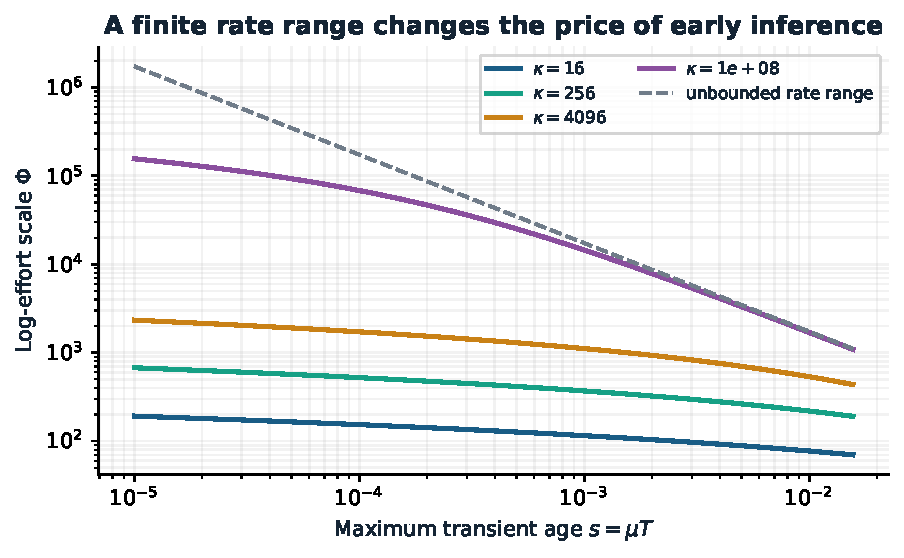
\includegraphics[width=.96\linewidth]{passive_programme/resource_crossover.pdf}
\caption{The proved scale $\Phi$ at $\varepsilon=1/64$, not exact numerical optimal effort. Finite rate ranges eventually enter the logarithmic-in-$1/s$ branch; an unbounded rate class retains the $1/s$ branch. Universal multiplicative factors are not plotted.}
\end{figure}

\section{The attaining operation}

\subsection{Finite ramp and integrated observations}

Choose $t_r=T/2$, $H=T/2$, and a plateau $U>0$. Raise the input monotonically from zero to $U$ by $t_r$ and then hold it. For peak cap $U_{\max}$ and slew cap $V_{\max}$, a linear ramp is allowed when
\[
U\leq\min\{U_{\max},V_{\max}T/2\}.
\]
Integration by parts gives, for $t\geq t_r$,
\begin{align}
y(t)&=U\int\lambda^{-1}\bigl[1-a_r(\lambda)e^{-\lambda(t-t_r)}\bigr]d\nu(\lambda),\\
a_r(\lambda)&=U^{-1}\int_0^{t_r}e^{-\lambda(t_r-v)}du(v)\in[0,1].\label{eq:ramp}
\end{align}
No impulse is used. The precise monotone rise profile need not be fitted: its unknown factor is already bounded. For a linear ramp $a_r=(1-e^{-\lambda t_r})/(\lambda t_r)$.

Choose degree $m\geq1$, $n=m+1$, and bin width $h=H/n$. Put
\begin{equation}
a=e^{-\Lambda h},\quad b=e^{-\mu h},\quad d=b-a,\quad
v=\frac{2-a-b}{d}>1,
\end{equation}
with $a=0$ when no upper rate is supplied. Define a Chebyshev residual
\begin{equation}\label{eq:residual}
R_m(z)=\frac{T_m((2z-a-b)/d)}{T_m(v)}
=\sum_{j=0}^m w_jz^j.
\end{equation}
The normalization $R_m(1)=1$ implies $\sum_jw_j=1$. Observe only the finite bin averages
\[
\bar Y_j=\frac{Y(t_r+(j+1)h)-Y(t_r+jh)}{h},\qquad j=0,\ldots,m,
\]
and return
\begin{equation}\label{eq:estimator}
\widehat S=\frac{\mu}{U}\sum_{j=0}^m w_j\bar Y_j.
\end{equation}
Negative weights are classical arithmetic, not negative physical spectral weights or an unbounded input waveform.

\begin{lemma}[Exact finite certificate]\label{lem:certificate}
The estimator has bias
\begin{equation}\label{eq:bias}
\E\widehat S-S
=-\int\frac{\mu}{\lambda}a_r(\lambda)
\frac{1-e^{-\lambda h}}{\lambda h}
R_m(e^{-\lambda h})d\nu(\lambda),
\end{equation}
so $|\E\widehat S-S|\leq\rho_m=1/T_m(v)$. Its variance and deterministic error amplification are
\begin{align}
V_m&=\frac{\mu^2\sigma^2}{U^2h}\sum_jw_j^2,\label{eq:variance}\\
\mathcal A_m:=\sum_j|w_j|
&=\frac{T_m((2+a+b)/d)}{T_m((2-a-b)/d)}.\label{eq:amplification}
\end{align}
In particular, bin errors $e_j$ add at most $(\mu/U)\mathcal A_m\max_j|e_j|$.
\end{lemma}
\begin{proof}
Let $z=e^{-\lambda h}$ and $\phi(\lambda h)=(1-z)/(\lambda h)$. Bin integration of~\eqref{eq:ramp} gives
\[
\E\bar Y_j=U\int\lambda^{-1}[1-a_r(\lambda)\phi(\lambda h)z^j]d\nu.
\]
Multiply by $\mu w_j/U$ and sum. Every factor preceding $R_m$ in the resulting bias integral is in $[0,1]$, while $|T_m|\leq1$ on $[-1,1]$. Independent Brownian increments give~\eqref{eq:variance}. All roots of $R_m$ lie in $(a,b)\subset[0,1)$, so its monomial coefficients alternate in sign. Consequently $\sum|w_j|=|R_m(-1)|$, proving~\eqref{eq:amplification}.
\end{proof}

If $\rho_m\leq\varepsilon/2$, averaging $M$ independent trials achieves failure probability at most $\alpha$ whenever
\begin{equation}\label{eq:repetitions}
M\geq\left\lceil\frac{8\mu^2\sigma^2}{U^2h\varepsilon^2}
\left(\sum_jw_j^2\right)\log\frac2\alpha\right\rceil.
\end{equation}
The compiler splits the error further to leave explicit room for digitization and other implementation errors. Each linear-ramp trial uses squared-drive effort $2U^2T/3$.

\subsection{Degree and coefficient bounds}

Set $s_H=\mu H$, $L_1=\log(4/\varepsilon)$ and
\begin{equation}\label{eq:degree}
m=\left\lceil\min\left\{\frac{\sqrt\kappa L_1}{2},
\frac{L_1^2}{2s_H}\right\}\right\rceil.
\end{equation}
For an unbounded rate class retain the second branch. If $\beta=\operatorname{arcosh}v$, then
\[
\beta=2\operatorname{artanh}\sqrt{\frac{1-b}{1-a}}
\geq\frac2{\sqrt\kappa},\qquad
\beta\geq\operatorname{arcosh}(2e^{\mu h}-1)\geq2\sqrt{\mu h}.
\]
The first inequality uses $(1-e^{-\kappa x})/(1-e^{-x})\leq\kappa$. The second follows by decreasing $a$ to zero and using $\cosh r\leq e^{r^2/2}$. Each branch of~\eqref{eq:degree} separately yields $m\beta\geq L_1$, since $m+1\leq2m$. Therefore
\[
\rho_m=\operatorname{sech}(m\beta)\leq2e^{-m\beta}\leq\varepsilon/2.
\]

For $x=\mu h<1$, $\kappa\geq2$,
\[
d=e^{-x}(1-e^{-(\kappa-1)x})\geq\frac1{4e}\min\{\kappa x,1\}.
\]
Since $T_m(z)\leq(2z)^m$ for $z\geq1$,
\begin{equation}\label{eq:coefficient-bound}
\log\mathcal A_m\leq m\log(8/d)
\leq C_0m[1+\log_+(1/(\kappa x))].
\end{equation}
When $s_H\sqrt\kappa/L_1\leq1$, the first degree branch has $m\asymp\sqrt\kappa L_1$ and $\kappa x\asymp s_H\sqrt\kappa/L_1$. In the other regime the second branch has $m\asymp L_1^2/s_H$ and $\kappa x\asymp(s_H\sqrt\kappa/L_1)^2$. These observations establish $\log\mathcal A_m=O(\Phi)$. The factors $m$, $\varepsilon^{-2}$ and fixed-confidence logarithms in~\eqref{eq:repetitions} are absorbed in the same exponent.

For complete integer-rounding control one may also impose $U\leq\sigma\mu/\sqrt T$. Then one extra rounded trial costs at most one normalized effort unit. Reducing $U$ only increases repetitions; arbitrary fixed positive peak and slew limits therefore do not change the exponent in the effort theorem. Their effects on elapsed time and repeated hardware remain real.

\section{The lower bound: positive indistinguishable systems}

Work in dimensionless rates $x=\lambda/\mu$ and time $t=\mu t_{\rm physical}$. The target is $\int x^{-1}d\nu$, and $x\in[1,\kappa]$.

\subsection{Finite positive spectra from classical approximation}

The established best reciprocal approximation error is \cite{kraus}
\begin{equation}\label{eq:best}
E_m(K):=\inf_{\deg p\leq m}\norm{x^{-1}-p}_{\infty,[1,K]}
=\frac{K-1}{2K}\left(\frac{\sqrt K-1}{\sqrt K+1}\right)^m.
\end{equation}
Take the $m+2$ alternating extrema $x_0<\cdots<x_{m+1}$ of its minimax error and put
\[
c_i=\left(\prod_{j\ne i}(x_i-x_j)\right)^{-1},\qquad
\omega=\frac{\sum_i c_i\delta_{x_i}}{\sum_i|c_i|}.
\]
Lagrange interpolation shows $\int p\,d\omega=0$ for every polynomial of degree at most $m$: the sum is its absent coefficient of degree $m+1$. The signs of $c_i$ alternate, as do the extremal errors. Choose the overall sign so that $\int x^{-1}d\omega=E_m(K)$. Its positive and negative masses are each $1/2$. Therefore
\begin{equation}\label{eq:witness}
\nu_+=2\omega_+,\qquad\nu_-=2\omega_-
\end{equation}
are probability measures matching moments $0,\ldots,m$ and satisfying
\begin{equation}
S(\nu_+)-S(\nu_-)=2E_m(K).
\end{equation}
Only $m+2$ rates in total are needed. The alternating extrema can be found from the explicit minimax polynomial by scalar root isolation. The supplied implementation uses its monotone phase formula and arbitrary-precision bisection. The exact mathematical construction is governed by~\eqref{eq:best}, not by a floating-point fit.

Every positive measure $\sum p_j\delta_{\lambda_j}$ has the physical deterministic realization $A=\operatorname{diag}(\lambda_j)$, $b_j=\sqrt{p_j}$. One circuit realization is a series connection of parallel RC branches with $C_j=1/p_j$, $R_j=p_j/\lambda_j$ in consistent units. Its impedance is $\sum_jp_j/(s+\lambda_j)$. All components are finite and positive. Intrinsic thermal noise requires a separate stochastic model; this deterministic realization alone does not remove it.

\subsection{Uniform early-time closeness}

Taylor expansion in $x-1\geq0$ gives
\[
\left|e^{-tx}-e^{-t}\sum_{j=0}^m\frac{[-t(x-1)]^j}{j!}\right|
\leq\frac{[t(K-1)]^{m+1}}{(m+1)!}.
\]
Moment matching eliminates the displayed polynomial, hence
\begin{equation}\label{eq:kernel-bound}
\eta:=\sup_{0\leq t\leq s}|k_+(t)-k_-(t)|
\leq2\left[\frac{es(K-1)}{m+1}\right]^{m+1}.
\end{equation}
The whole early step-response difference is at most $s\eta$.

Now choose
\begin{equation}\label{eq:lower-choice}
L_0=\log\frac1{4\varepsilon},\quad
K=\min\left\{\kappa,\left(\frac{L_0}{8es}\right)^2\right\},\quad
m=\left\lfloor\frac{\sqrt K L_0}{4}\right\rfloor.
\end{equation}
The theorem's ranges imply $K\geq16$ and $m+1\geq2$. For $q=(\sqrt K-1)/(\sqrt K+1)$, $\log q\geq-3/\sqrt K$, so
\begin{equation}\label{eq:gap}
S(\nu_+)-S(\nu_-)
\geq\frac{15}{16}e^{-3m/\sqrt K}
\geq\frac{15}{16}(4\varepsilon)^{3/4}>4\varepsilon.
\end{equation}
Meanwhile $es(K-1)/(m+1)\leq4es\sqrt K/L_0\leq1/2$. In particular,
\[
-\log\left(2\left[\frac{es(K-1)}{m+1}\right]^{m+1}\right)
\geq\frac{\sqrt K L_0}{8}\log\frac{L_0}{4es\sqrt K}.
\]
If $K=\kappa$ this is $\Omega(\sqrt\kappa L_0\log(1+L_0/(s\sqrt\kappa)))$; otherwise it is $\Omega(L_0^2/s)$. Since $L/2\leq L_0\leq L$, in both cases $\eta\leq e^{-c_0\Phi}$ after adjusting universal constants.

The hard family has $O(\min\{\sqrt\kappa L,L^2/s\})$ total modes. In the broad-rate regime its maximum physical rate is $O(L^2/(\mu T^2))$. Hidden order and rate range are thus explicit growing features of the worst-case family. This is not a claim that one fixed small device develops that exponential dependence as its observation deadline changes.

\begin{figure}[htbp]
\centering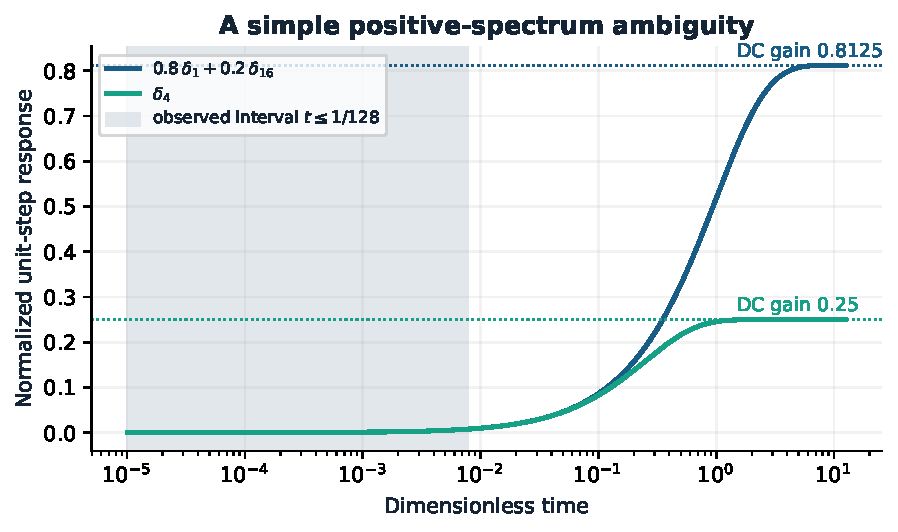
\includegraphics[width=.96\linewidth]{passive_programme/simple_witness.pdf}
\caption{The simplest exact example uses rates $1,4,16$. The measures $0.8\delta_1+0.2\delta_{16}$ and $\delta_4$ match mass and first moment, while their static gains are $0.8125$ and $0.25$. Higher-order versions establish the joint asymptotic law.}
\end{figure}

\subsection{Why all causal forcing is covered}

Return to physical time. If the impulse-response difference is at most $\eta$ on $[0,T]$, Young's convolution inequality gives
\begin{equation}
\norm{(k_+-k_-)*u}_{L^2[0,T]}\leq T\eta\norm{u}_2.
\end{equation}
Conditional on the same observed history, a fixed causal algorithm chooses the same input under both models. Gaussian change of measure therefore yields
\begin{equation}\label{eq:KL}
\KL(P_+\Vert P_-)
\leq\frac{1}{2\sigma^2}\E_+\sum_i\norm{(k_+-k_-)*u_i}_2^2
\leq\frac{\eta^2T^2 E}{2\sigma^2}
=\frac{\eta^2s^2\mathcal B}{2}.
\end{equation}
The deterministic effort cap supplies integrability; stopping is handled by stopping the observation process. Independent randomized choices are included in the transcript. No restriction to fixed waveforms, linear estimators or explicit model reconstruction is used.

An estimator accurate to $\varepsilon$ under both separated targets gives a binary test by thresholding between them. If failure is at most $\alpha<1/2$, binary data processing implies
\begin{equation}\label{eq:confidence-lower}
\mathcal B\geq
\frac{2\operatorname{kl}(1-\alpha,\alpha)}{s^2\eta^2},\qquad
\operatorname{kl}(1-\alpha,\alpha)
=(1-2\alpha)\log\frac{1-\alpha}{\alpha}.
\end{equation}
Combining this with~\eqref{eq:kernel-bound}--\eqref{eq:lower-choice} proves the lower half of Theorem~\ref{thm:main}. At fixed confidence, the attaining construction proves the upper half. This closes the stated minimax problem in logarithmic order.

\section{Exact rational compiler and executed evidence}

\subsection{A finite certificate without exponential endpoint evaluation}

For rational inputs $\mu,\Lambda,T$, replace the exact exponential interval by
\begin{equation}\label{eq:rational}
a=\max\{0,1-\Lambda h\},\qquad b=\frac1{1+\mu h}.
\end{equation}
The elementary inequalities $1-x\leq e^{-x}\leq(1+x)^{-1}$ give
\[
a\leq e^{-\Lambda h}\leq e^{-\lambda h}\leq e^{-\mu h}\leq b<1.
\]
The same residual has exactly rational weights, exactly rational bias bound, exactly rational $\ell_1$ norm and exactly rational variance. The supplied compiler increases $m$ until its exact bias check passes; it does not claim a least-degree search. The wider interval preserves the asymptotic rate, although it can increase finite costs.

The recurrence for $T_m$ uses $O(m^2)$ arithmetic operations for all coefficients. Bit complexity also includes their growing numerator and denominator lengths. It is not valid to count large-precision arithmetic as unit-cost hardware. Working precision and readout precision must accommodate $\log\mathcal A_m$, because large positive and negative terms cancel.

\subsection{Concrete sufficient recipe}

For $\mu=1$, $\Lambda=16$, $T=0.1$, $\varepsilon=1/16$, $U=\sigma=1$ and confidence $0.95$, the exact rational implementation returns:
\begin{center}
\begin{tabular}{lr}
\toprule
Quantity&Returned value\\\midrule
Polynomial degree / bin count&$10$ / $11$\\
Uniform bias bound&$0.0122397272$\\
$\log_{10}\mathcal A_m$&$18.3946217$\\
$\log_{10}$ sufficient repetitions&$43.1362787$\\
$\log_{10}$ normalized squared-drive effort&$41.9601875$\\
$\log_{10}$ allowed bin digitization error&$-20.2008017$\\
Exact sum of weights&$1$\\\bottomrule
\end{tabular}
\end{center}
This finite certificate is valid outside the deliberately narrower domain used to state the asymptotic theorem. The astronomical repetition count is a sufficient bound for this specified estimator and noise level, not an evaluated optimum or a simulated laboratory run. It demonstrates why an attained mathematical operation need not be practical.

\subsection{Verification scope}

The package includes the following executed evidence:
\begin{itemize}
\item Exact rational normalization, amplification and stopping identities for the compiler; 12 finite parameter recipes.
\item Sixty positive finite spectra with dimensions $1,2,8,32,128$, evaluated at 90--121 decimal digits. Every estimated bias stayed within its analytic bound. Separate time-domain integrations checked the actual finite-ramp/bin operation.
\item Four positive moment-matched families evaluated at 250 decimal digits. Saved spectra carry 270 significant digits; a reload audit reproduced the checks from the serialized values.
\item An independent 100-digit challenge grid of 120 parameter combinations, including $\varepsilon=e^{-1000}$, $s=10^{-10}$ and an unbounded rate range. The analytic parameter inequalities passed every listed case. Those observations are not estimates of universal constants.
\end{itemize}

One hard pair has $\kappa=4096$, $s=1/2048$, $\varepsilon=1/256$, and 68 total support points. Its analytical target-gap formula evaluates to about $0.127083358499084$, while~\eqref{eq:kernel-bound} certifies a whole-interval impulse-response difference at most $1.6356\times10^{-73}$. Its sampled difference was smaller, about $1.66\times10^{-116}$; only the former is the uniform bound. Numerical moment residuals near $10^{-251}$ corroborate the exact moment identity, but the mathematical equality follows from interpolation, not from the finite residual.

The upper witness script uses the ideal step/bin formula and exact exponential endpoints evaluated at high precision. The separate rational compiler uses a finite ramp, rational enclosure and a finer implementation error split. Their finite counts should not be conflated.

\section{Physical requirements, uncertainty and reuse}\label{sec:resources}

\textbf{Preparation.} The minimax interface grants zero-state trials, which strengthens its lower bound. An actual implementation with initial norm at most $B$ can instead wait passively. After a wait $W$, the residual norm is at most $Be^{-\mu W}$ and its contribution to the estimator is bounded by $(\mu/U)\mathcal A_mBe^{-\mu W}$. A preparation error budget $\varepsilon_p$ is met by
\begin{equation}
W\geq\frac1\mu\left[\log\frac{\mu\mathcal A_mB}{U\varepsilon_p}\right]_+.
\end{equation}
After a bounded-input trial, $B$ can be updated using $\norm{x(t)}\leq e^{-\mu t}B+U/\mu$. Reset time may be of order $\Phi/\mu$, far longer than the interrogation horizon. An observed long reset trace is extra information and changes the short-age comparison. A repeated experiment does not deliver a free total-time advantage over waiting for equilibrium.

\textbf{Unknown initial conditions.} A separate upper construction can randomize the sign of the entire ramp after the initial state is fixed, then multiply the result by that sign. The homogeneous initial-state response has zero conditional mean; if $\norm{x_0}\leq B$, its sub-Gaussian contribution is bounded using $(\mu\mathcal A_mB/U)^2$. This adds repetitions instead of demanding exact zero preparation. It does not extend the lower theorem to unrestricted long-time reuse of one plant.

\textbf{Control.} The input can have finite peak and finite slew. A common amplitude miscalibration scales the result; an unknown but monotone rise is covered by~\eqref{eq:ramp}. Nonmonotone leakage, drift, nonlinear response or changing $A$ need their own bounds. The source must remain in the declared linear regime throughout all trials.

\textbf{Readout.} Finite integration bins are essential to the construction. Their rate is $(m+1)/H$. A fixed detector bandwidth can prevent an arbitrarily short $T$. A Gaussian read-noise model is a premise, not an acquired fact. Integrator settling, digitization, saturation and clock errors must be allocated a finite budget. Arbitrary bin-dependent bias is amplified by $\mathcal A_m$; repeated observations do not remove it. A common constant offset is less damaging because $\sum w_j=1$.

\textbf{Thermal noise.} The main optimality theorem assumes parameter-independent additive sensor noise. It does not automatically cover an arbitrary thermal plant. As a separate attainable upper extension, consider
\[
dx=(-Ax+bu)dt+\sqrt{2\Theta A}\,dB_t
\]
from a zero state, with $\Theta$ known and thermal Brownian noise $B_t$ independent of sensor noise $W_t$. The thermal output covariance is
\[
\operatorname{Cov}(y(t),y(v))
=\Theta\{k_\nu(|t-v|)-k_\nu(t+v)\},
\]
whose magnitude is at most $\Theta$. Thus the estimator's variance increases by at most
\[
(\mu/U)^2\Theta\mathcal A_m^2.
\]
Independent thermal trials add sufficient normalized effort of order
\[
\frac{\Theta T}{\sigma^2}\mathcal A_m^2\varepsilon^{-2}\log(1/\alpha).
\]
At fixed $\Theta T/\sigma^2$, this does not change the upper exponent. This calculation is not an all-adaptive lower bound for the thermal interface: its parameter-dependent fluctuation statistics may supply further information. A different OU model with noise $\sqrt{2\Theta I}\,dB_t$ and an equilibrium start has variance $\Theta b^\top A^{-1}b$, directly revealing the target through equal-time fluctuations. These are different physical premises.

\textbf{Reuse and hardware.} Serial repetitions cost every interrogation and reset. Parallel repetitions cost identical specimens, readout channels and preparation hardware. Calibration must persist across them. The final scalar estimate can be reused to answer static queries about the same unchanged system; it does not certify new interventions that alter its dynamics. There is no catalytic hardware or protection claim. In a noisy implementation, ordinary bounds on systematic drift and stored digital data must be supplied.

\textbf{Hard-family realization.} The finite RC construction proves existence within the passive model. A laboratory pair reproducing exponentially close traces would require correspondingly precise component values and thermal/noise control. No such apparatus was built or tested. The theorem is a worst-case statement; it does not claim typical devices are this hard.

\section{Strongest existing approaches and the actual addition}

\begin{center}\small
\begin{tabular}{p{.24\linewidth}p{.68\linewidth}}
\toprule
Approach&Comparison\\\midrule
Direct settling&For a unit step, the normalized residual bias is at most $e^{-\mu T}$. Waiting $O(\mu^{-1}\log(1/\varepsilon))$ is often far cheaper than the short-age estimator. It is available whenever the horizon restriction is lifted.\\[3pt]
Optimal extrapolation&The attaining operation uses ordinary Chebyshev extrapolation. The result establishes its logarithmic minimax order at this interface; it does not beat the strongest ordinary same-access method.\\[3pt]
Full system identification&Also permitted by the lower bound. Learning an entire spectrum cannot uniformly evade the indistinguishable positive families. Extra finite-order or separation assumptions can change the answer.\\[3pt]
Matrix and hidden-state access&Ordinary linear solvers can exploit this stronger access. It is absent from the scalar-port experiment and is not ruled out by the theorem.\\[3pt]
Equilibrium fluctuation data&May encode the target directly under an appropriate thermodynamic model. Preparing independent equilibrium states and specifying the fluctuation law are separate resources.\\\bottomrule
\end{tabular}
\end{center}

Brown and Grabovsky prove a precise extrapolation exponent for completely monotone functions, $(2/\pi)\arcsin(1/x_0)$, in a relative $L^2$ formulation at a fixed extrapolation point \cite{brown}. That work already establishes that positivity does not make extrapolation well conditioned. The present derivation targets a normalized inverse moment, includes a finite rate-range parameter, supplies uniform joint short-age/high-accuracy bounds, and connects them to arbitrary causal forcing and an attaining finite-ramp operation.

The reciprocal minimax formula and the Chebyshev residual are not new \cite{kraus}. Donoho's framework already explains why moduli of continuity and carefully chosen linear estimators govern many convex functional-estimation problems \cite{donoho}. General inverse-Laplace instability is likewise established \cite{epstein}. The possible research contribution is the combined statement and proof at the specified interface; establishing its historical novelty would require further specialist comparison.

\section{Relation to preserved Astra work}

The prior homogeneous tracial partial-SWAP programme is retained at its earned scope: its arbitrary-accuracy block compressor, exact acquisition-loss ledger, earlier prefix converses and reverse decoder remain available. The unrestricted optimal joint memory/processing law is not resolved here.

The new passive theorem does not inherit the prior private-timing preparation result without conditions. That result treats a retained loaded LTI plant with a local dissipation bound and finite initial energy, and earns finite-horizon prediction without hidden equilibration. The present theorem instead assumes a positive relaxation spectrum with supplied gap and rate range and targets the static functional. Similarly, the earlier passive-current obstruction without a relaxation floor remains distinct from a quantitative law \emph{given} such a floor. Exact governing Astra routes and the pinned revision are recorded in the bundle \cite{astra}.

\section{Independent quantum companion}

One independent route produced a completed scoped extension, preserved separately. A single arbitrary unknown qubit occupies one site of an $n$-spin source; the other spins start tracial. Each cycle applies a fresh uniformly random $n$-qubit Clifford, with its full label available to the receiver, and then local partial-SWAP collisions with fresh tracial carriers. Define
\[
\gamma_n=\frac{(1+3\sin^4\theta)^n-1}{4^n-1},\qquad
\eta_n=\frac{(1+3\cos^2\theta)^n-1}{4^n-1}.
\]
After $q$ cycles a physical mixed-dummy inverse reader has exact averaged half-diamond error
\[
\varepsilon_{\rm inv}=\frac34(1-\gamma_n)^q,
\]
while every decoder, even with all outputs and full Clifford records, obeys
\[
\varepsilon_{\rm opt}\geq
\frac34\left(1-\sqrt{1-(1-\gamma_n)^q}\right).
\]
The source channel \emph{with the public key retained} is within at most $\tfrac32\eta_n^q$ of its tracial replacer in half diamond distance. At fixed angle both $\gamma_n$ and $\eta_n$ decay exponentially in $n$, giving rapid source forgetting and exponentially slow output acquisition. These are physical randomized-channel statements, with a further high-probability fixed-key obstruction in the companion note, not assertions about every individual schedule.

The proof tracks orthogonal Pauli histories. A local active source Pauli exports its complete support with squared weight $\sin^4\theta$; fresh Clifford transitivity makes the per-cycle extinction probability exactly $\gamma_n$. Tracial Petz reversal gives the inverse reader; a Cauchy--Schwarz Bell-fidelity bound gives the universal converse. Local two-site random Clifford layers produce the known occupation process with effective death probability $p=\sin^4\theta$.

Weinstein, Kelly, Marino and Altman already established the radiative scrambling mechanism, inverse-circuit reader and operator-survival fidelity for random full-SWAP emission \cite{weinstein}. The companion is a coherent-collision and finite-size extension with an all-decoder bound, not a new mechanism. Its displayed reader stores $nq$ output qubits and pays source scrambling, inversion, routing, precision and protection. It does not solve the original memory problem. Fifteen dense finite-circuit checks and an exhaustive two-qubit symplectic transitivity check are included in its separate files.

\section{What is completed and what is not}

The completed mathematical programme supplies a matching joint resource law, an attainable bounded-input operation, finite positive lower witnesses, an exact rational compiler and a reproducible internal checking record. It establishes a precise limit on when early observations can support a late-response conclusion, even under sophisticated active experimental design.

It does not establish a new generally useful physical discovery machine, a practical speed advantage over optimal extrapolation, a universal thermodynamic speed limit, a theorem about typical materials, an acquired spectral gap, an externally verified first discovery, or civilisation-changing impact. Those conclusions would exceed the result. The durable gain is a complete, inspectable decision about this structured scientific question and reusable machinery for compiling and falsifying early-response claims.

\appendix
\section{Reproducing the artifacts}

The core compiler uses Python's standard library and exact \texttt{Fraction} arithmetic. Numerical witness checks use \texttt{mpmath}; the spectrum checks and figures additionally use \texttt{numpy} and \texttt{matplotlib}. From the package root:
\begin{verbatim}
python3 passive_programme/response_compiler.py \
  --mu 1 --upper 16 --horizon 1/10 --epsilon 1/16 \
  --alpha 1/20 --output response_certificate.json
python3 passive_programme/verify_compiler.py
python3 passive_programme/check_bandwidth_witnesses.py
python3 passive_programme/audit_grid.py
python3 quantum_companion/verify.py
\end{verbatim}
The default compiler certificate uses a quarter of the accuracy for bias, a quarter for statistical error, a quarter for digitization and leaves a quarter for arithmetic/control/preparation. It provides sufficient counts under the declared statistical model. It does not perform experiments. Its \texttt{--max-degree} cap is an explicit implementation limit, not a mathematical impossibility bound.

Read \texttt{README.txt}, the proof notes, the independent audit, and the JSON checking records before interpreting a number. The report's finite numerical recipes have their own inputs; they are not all instances of the same confidence/error split. The integrity manifest identifies the distributed files.

\begin{thebibliography}{9}
\bibitem{brown} H.~J. Brown and Y.~Grabovsky, \emph{On Feasibility of Extrapolation of Completely Monotone Functions}, SIAM J. Math. Anal. \textbf{56}(6), 7713--7747 (2024). DOI: \href{https://doi.org/10.1137/24M1652325}{10.1137/24M1652325}. \href{https://arxiv.org/html/2401.15178v2}{Primary manuscript}. The displayed journal year is 2024.
\bibitem{kraus} J.~K. Kraus, P.~S. Vassilevski and L.~T. Zikatanov, \emph{Polynomial of best uniform approximation to $x^{-1}$ and smoothing in two-level methods}, Comput. Methods Appl. Math. \textbf{12}(4), 448--468 (2012). DOI: \href{https://doi.org/10.2478/cmam-2012-0026}{10.2478/cmam-2012-0026}. \href{https://arxiv.org/pdf/1002.1859}{arXiv:1002.1859v3}.
\bibitem{donoho} D.~L. Donoho, \emph{Statistical Estimation and Optimal Recovery}, Ann. Statist. \textbf{22}(1), 238--270 (1994). DOI: \href{https://doi.org/10.1214/aos/1176325367}{10.1214/aos/1176325367}. \href{https://web.stanford.edu/dept/statistics/cgi-bin/donoho/wp-content/uploads/2018/08/SEOR.pdf}{Author-hosted primary paper}.
\bibitem{epstein} C.~L. Epstein and J.~Schotland, \emph{The Bad Truth about Laplace's Transform}, SIAM Rev. \textbf{50}(3), 504--520 (2008). DOI: \href{https://doi.org/10.1137/060657273}{10.1137/060657273}.
\bibitem{weinstein} Z.~Weinstein, S.~P. Kelly, J.~Marino and E.~Altman, \emph{Scrambling Transition in a Radiative Random Unitary Circuit}, Phys. Rev. Lett. \textbf{131}, 220404 (2023). DOI: \href{https://doi.org/10.1103/PhysRevLett.131.220404}{10.1103/PhysRevLett.131.220404}. \href{https://arxiv.org/html/2210.14242v2}{Primary manuscript}.
\bibitem{astra} Astra Research Knowledge, pinned revision \texttt{c11d35bd2e07116e214b4388302595cfedbd770e}. Governing direct returns: \texttt{2026-11-05-p2-predictive-preparation}, \texttt{2026-11-05-p3-correlated-reliability/transport-certification.md}, and the preserved \emph{joint\_recovery\_continuation} report. \href{https://github.com/harjassand/astra-research-knowledge/tree/c11d35bd2e07116e214b4388302595cfedbd770e/research/returns}{Pinned source routes}. These are scoped inputs, not evidence of external priority for the present result.
\end{thebibliography}
\end{document}
